\section{Q\# og Implementasjon av kvantevandringer}

    I dag finnes det flere alternativer for å programmere kvantealgoritmer med høynivå språk. I Python skrives det flere moduler som IBM sitt \emph{qiskit} og \emph{openql}. I Haskell finnes det flere domene spesifikke språk som \emph{quipper} og \emph{quantum IO monad}. Microsoft har utviklet \emph{Q\#} som er et dotnet basert språk, inspirert av \emph{quantum IO monad}, men har semantikk fra C\# og F\#. Noen av disse språkene som \emph{qiskit} og \emph{Q\#} er skrevet slik at man kan bruke bedriftene sine Kvanteberegnings løsninger.

    I dette prosjektet har jeg valgt å bruke Q\# for å eksperimentere med kvantealgoritmene. Figur \ref{fig:d-reg}, \ref{fig:Simp graf} og \ref{fig:shuriken} får alle implementert en kvantevandringsalgoritme. Vi ser litt hvordan algoritmene ser ut i et annet perspektiv, sammen med noe eksperimentell data. Implementasjonene av algoritmene tar i tillegg å fremhever noen interessante problemstillinger ved slike implementasjoner.

    \subsection{Q\# intro}

        Q\# er et sterkt typet språk, dette vil si at man ikke kan gjøre implisitt casting mellom typer, og alle funksjoner skal ha en entydig type signatur. De typene som er primitive for språket er String, Int, Double, =>, Qubit, Result, Unit og Array. String, Int, Double og => er kjent fra andre programmeringsspråk, nemlig tekst, heltall, flyttall og funksjoner. Typene som skiller Q\# fra andre språk er Qubit, Result og Unit. En term av typen Qubit representerer en qubit i et kvantesystem. På disse kan vi utføre operasjoner som har typen Qubit => Unit. Unit typen fanger effekter som utføres på qubits eller filer. Typen Unit kan ligne på Void typen i C, men den er analog til IO monaden i Haskell. Typen Result har termene Zero og One, og denne representerer en måling av et system. Den siste typen Array er en funktor av typer. Dette vil si at det er en abstrakt type som opererer på andre typer. F.eks. kan vi lage Int[] og Qubit[], som er lister av heltall og lister av qubits.

        For å beskrive hvordan Q\# er det vedlagt introduksjons kode i appendix A. Denne forklarer hvordan man konstruerer funksjoner, deklarerer variabler og bruke kontroll uttrykk.

        All koden som er skrevet til dette prosjektet ligger opplastet på \url{https://github.com/celestialcry/quantum_walks}. Den relevante koden ligger i Program.qs. Bemerk at koden er kjørt fra Python via filen host.py.

    \subsubsection{Grover's algoritme og Amplitude forsterkning}
    
        Vi vil starte med å beskrive Grover's algoritme i Q\#. For dette trenger vi å kunne konstruere faseorakler. Dette gjør vi med teknikken som er beskrevet med figur \ref{fig:faseorakel}. Akkurat som i figuren konjugerer vi en hjelpequbit med $HX$, og anvender oraklet.
        
        \begin{Verbatim}[gobble=2, numbers=left, frame=lines,
            framesep=3mm,
            label={[Beginning of code]End of code}]
            // Oracle Conversion
            operation MarkingAsPhase(register : Qubit[], 
                                    oracle : (Qubit[], Qubit) => Unit is Adj) 
                                    : Unit is Adj {
                use target = Qubit();
                within {
                    X(target);
                    H(target);
                }
                apply {
                    oracle(register, target);
                }
            }

            function MarkingToPhase(oracle : (Qubit[], Qubit) => Unit is Adj) 
                                    : (Qubit[] => Unit is Adj) {
                return MarkingAsPhase(_, oracle);
            }
        \end{Verbatim}

        
        $R$ operatoren er definert som $2|0\rangle^{\otimes n}\langle 0|^{\otimes n} - I$. Siden å modifisere den globale fasen ikke endrer utfallet endrer vi operatoren $R$ til $I - 2|0\rangle^{\otimes n}\langle 0|^{\otimes n}$ for simpelhetens skyld.

        \begin{Verbatim}[gobble=2, numbers=left, frame=lines,
            framesep=3mm,
            label={[Beginning of code]End of code}]
            // Zero Oracle
            operation MarkingZero(register : Qubit[], target : Qubit) : Unit
            is Adj + Ctl {
                within {
                    ApplyToEachCA(X, register);
                }
                apply {
                    Controlled X(register, target);
                }
            }

            operation R(register : Qubit[]) : Unit is Adj {
                MarkingToPhase(MarkingZero)(register);
            }
        \end{Verbatim}

        Nå har vi alle byggeklossene til å definere en Grover's iterate og dermed bygge Grover's algoritme.

        \begin{Verbatim}[gobble=2, numbers=left, frame=lines,
            framesep=3mm,
            label={[Beginning of code]End of code}]
            // One Grover's iterate
            operation GroversIterate(register : Qubit[], 
                                    phaseOracle : Qubit[] => Unit is Adj) 
                                    : Unit is Adj {
                phaseOracle(register);
                within {
                    ApplyToEachCA(H,register);
                }
                apply {
                    MarkingToPhase(MarkingZero)(register);
                }
            }

            // Grover's algorithm
            operation GroversAlgorithm(register : Qubit[], 
                                    phaseOracle : Qubit[] => Unit is Adj, 
                                    time : Int) 
                                    : Unit {
                // Initiate initial state
                ApplyToEachCA(H,register);

                // Running Grover's algorithm
                for i in 1..time {
                    GroversIterate(register, phaseOracle);
                }
            }
        \end{Verbatim}

        Denne funksjonen tester vi på bitstringen $0100010000000010$. Målet er dermed å oppdage at den 2e, 6e og 14e bitten er en 1er. Vi kan regne ut antallet iterasjoner vi skal bruke er $k = 1$. Grover's algoritme presterer veldig bra, som man kan se i figur \ref{fig:Grover's}

        \begin{figure}
            \begin{center}
                \caption{Grover's algoritme kjørt på $0100010000000010$}
                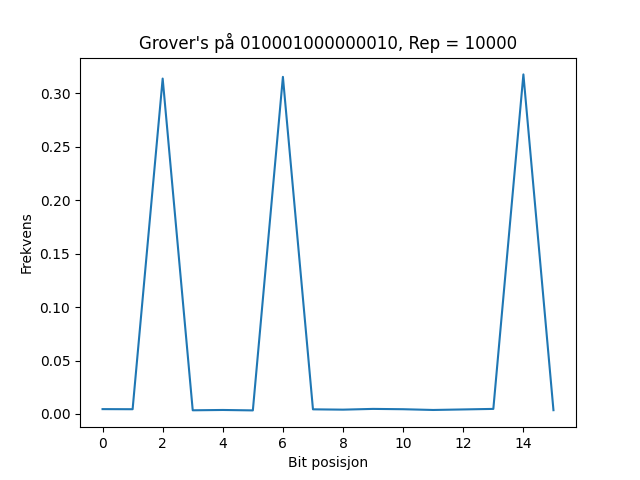
\includegraphics[scale=0.5]{Grovers.png}
                \label{fig:Grover's}
            \end{center}
        \end{figure}

        Vi kan generalisere Grover's algoritme til amplitudeforsterkningsteknikken ved å ha alle operatorene som input. Den implementeres helt analogt som Grover's algoritme.

        \begin{Verbatim}[gobble=2, numbers=left, frame=lines,
            framesep=3mm,
            label={[Beginning of code]End of code}]
            // Amplitude amplification technique
            operation AmplitudeAmplification(register : Qubit[], 
                                            outputOperator : (Qubit[] => Unit is Adj), 
                                            phaseOracle : (Qubit[] => Unit is Adj), 
                                            time : Int) 
                                            : Unit is Adj {
                for i in 1..time {
                    outputOperator(register);
                    phaseOracle(register);
                }
              }
        \end{Verbatim}

    \subsection{Kvantevandringer}

        Vi vil se på noen simuleringer av de kvantevandringene som vi har laget tidligere i rapporten. Den initielle tilstanden til kvantevandringen påvirker utfallet sterkt, og dette er en av effektene vi vil se på. I position-coin notation vil vi også se på effekten av å bruke forskjellige mynter. Til slutt skal vi gjøre et kvantesøk eksperiment. Merk at de grafene vi ser på er endelige og har nødvendigvis ikke en symmetri som gjør vandringene enklere å studere.

        Diskrete kvantevandringer på ubegrensede grafer som linjen og gitteret i 2 dimensjoner har blitt omfattende studert i andre verk (se \cite{portugal_2019} og \cite{Venegas_Andraca_2012}). Under rimelige antagelser kan man finne analytiske løsninger av posisjonen til kvantepartikkelen. Dette er gjort på den ubegrensede linjen, det ubegrensede 2 dimensjonale gitteret, sirkelen, det begrensede 2 dimensjonale gitteret og hyperkuben.

        Videre legges det ikke til spesifikke kodesnutter, men mer abstrakt kode. For å finne konkretiseringen av disse kodesnuttene så finner man resten av koden i github repoet nevnt over.
    
            \begin{figure}
                \begin{center}
                    \caption{Kvantevandring over \ref{fig:d-reg}}
                    \label{fig: d-reg vandring}
                    \begin{subfigure}{0.65\textwidth}
                        \begin{center}
                            \caption{start i node 0, Hadamardmynten}
                            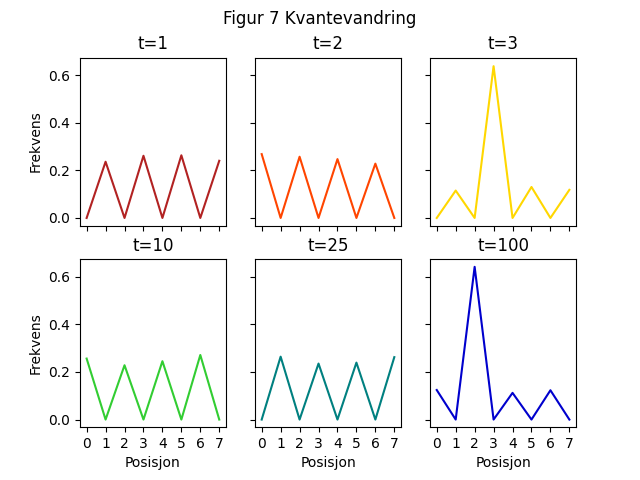
\includegraphics[scale=0.5]{Fig7Start0.png}
                        \end{center}
                    \end{subfigure} 
                \end{center}
                \begin{center}
                    \begin{subfigure}{0.8\textwidth}
                        \begin{center}
                            \caption{start uniformt, Hadamardmynten}
                            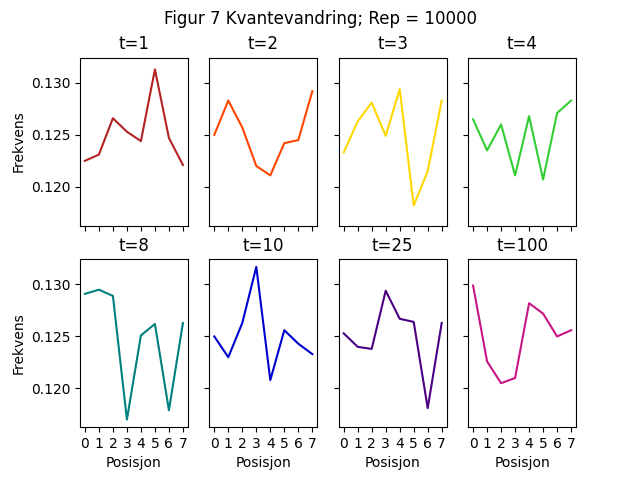
\includegraphics[scale=0.5]{Fig7Hadamard.png}
                        \end{center}
                    \end{subfigure}
                \end{center}
                \begin{center}
                    \begin{subfigure}{0.8\textwidth}
                        \begin{center}
                            \caption{start uniformt, Grovermynten}
                            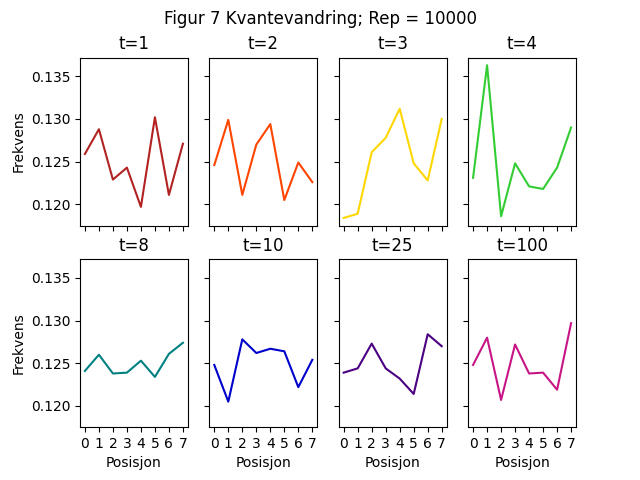
\includegraphics[scale=0.5]{Fig7Grover.png}                        
                        \end{center}
                    \end{subfigure}
                \end{center}
            \end{figure}

        \subsubsection{Position-coin notation}

            Vi starter med å se på position-coin notation. Denne kvantevandringen foregår over Hilbertrommet $\mathcal{H}_V\otimes \mathcal{H}_C$, disse rommene er representert som \emph{position} og \emph{color}. Den abstrakte koden for denne kvantevandringen kan man se under.

            \begin{Verbatim}[gobble=2, numbers=left, frame=lines,
                framesep=3mm,
                label={[Beginning of code]End of code}]
                operation PoistionCoinWalk(position : Qubit[], 
                                        color : Qubit[], 
                                        Shift : ((Qubit[],Qubit[]) => Unit is Adj), 
                                        Coin : (Qubit[] => Unit is Adj), 
                                        steps : Int) 
                                        : Unit is Adj {
                    for i in 1..steps {
                        Coin(color);
                        Shift(position, color);
                    }
                }
            \end{Verbatim}

            For å implementere enn konkret kvantevandring trenger vi å bestemme hva operatorene Shift og Coin er. Vi starter med å studer Coin. Dimensjonen som denne operatoren operer over er $d$, det kant kromatiske tallet. Mynten kan være en vilkårlig operator som virker på dette rommet. Naturlige valg er mynter som har uniforme sannsynlighetsfordelinger, derav Hadamardmynten, Grovermynten og Fouriermynten.
            
            Shift operatoren er mer interessant for denne strukturen. Siden vi bruker flip-flop operatorene har vi faktisk at Shift operatoren er unikt bestemt av fargeleggingen av kantene. Dette gjør at strukturen til grafen er totalt fanget av implementasjonen til Shift operatoren.

            Som vi ser i figur \ref{fig: d-reg vandring}, så har kvantevandringene en del tilfeldige egenskaper etter hvordan de beveger seg. Vi ser f.eks. at i del (a) hvordan vandringen er nesten uniform i de to første stegene, men i steg 3 for den en topp. Denne toppen skyldes nok kansellering og konstruksjon av de forskjellige fasene som blir sendt rundt. I figur (b) og (c) er disse effektene enda tydeligere, ettersom grafene er mer eller mindre tilfeldig. Det er vanskelig å si om disse effektene skyldes av interferens, eller om de skyldes av feil i implementasjon eller kjørefeil under simuleringen.

            I figur \ref{fig: d-reg vandring} (b) bruker vi Hadamardmynten og (c) bruker vi Grovermynten. Til sammenligning kan vi se at interferensen opptrer forskjellig. Karakteristikken til kvantevandringene er vanskelig å skille på, ettersom alt virker tilfeldig. I figur \ref{fig: d-reg vandring} (a) er det mye tydligere å se at enkelte mønstre gjentar seg. Dette motiverer quasi-periodisiteten til kvantevandringene.

            \begin{figure}
                \begin{center}
                    \caption{Kvantevandring over \ref{fig:Simp graf}}
                    \begin{subfigure}{0.6\textwidth}
                        \begin{center}
                            \caption{start i node $0$}
                            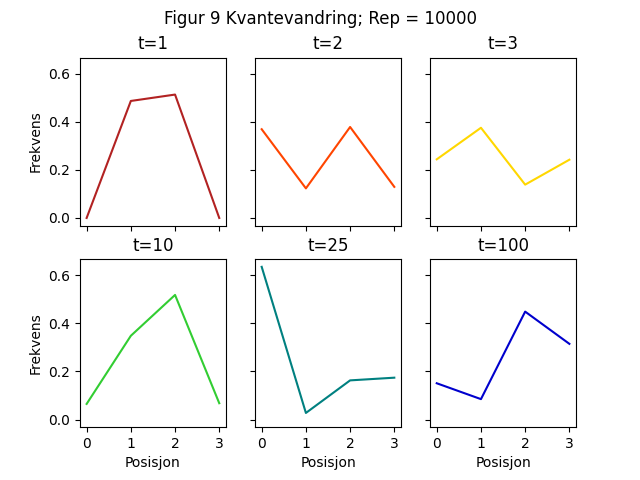
\includegraphics[scale=0.5]{Fig9Start0.png}
                        \end{center}
                    \end{subfigure} \\
                    \begin{subfigure}{0.6\textwidth}
                        \begin{center}
                            \caption{start uniformt}
                            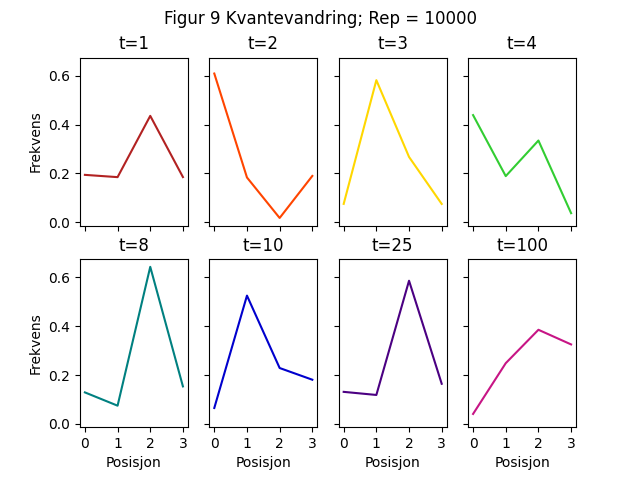
\includegraphics[scale=0.5]{Fig9Hadamard.png}
                        \end{center}
                    \end{subfigure}
                    \label{fig:simp vandring}
                \end{center}
            \end{figure}

        \subsubsection{Arc notation}

            I arc notation foregår kvantevandringen over Hilbertrommet $\mathcal{H}_V\otimes\mathcal{H}_V$, dette er representert som \emph{present} og \emph{past}. Den abstrakte definisjonen for en slik kvantevandring er gitt under.

            \begin{Verbatim}[gobble=2, numbers=left, frame=lines,
                framesep=3mm,
                label={[Beginning of code]End of code}]
                // Arc flip-flop operator (MultiSWAP gate)
                operation ArcFlipFlop(present : Qubit[], past : Qubit[]) : Unit
                is Adj {
                    // Get qubit length
                    let presentSize = Length(present);
                    let pastSize = Length(past);

                    // past and present qubit size should be the same
                    Fact(presentSize == pastSize, "Not a valid format");

                    // Switch wires
                    for i in 0..(presentSize-1) {
                        SWAP(present[i], past[i]);
                    }
                }

                // The coin operator is determined by each nodes neighbors
                operation ArcWalk(present : Qubit[], 
                                past : Qubit[], 
                                Coin : ((Qubit[],Qubit[]) => Unit is Adj), 
                                steps : Int) 
                                : Unit is Adj {
                    for i in 1..steps {
                        Coin(present, past);
                        ArcFlipFlop(present, past);
                    }
                }
            \end{Verbatim}

            Som vi kan se i den abstrakte beskrivelsen av arc notation kvantevandringen under trenger vi ikke å eksplisitt oppgi en Shift operator. Denne operatoren er definert som ArcFlipFlop, og er ekvivalent med den symmetriske isomorfien av tensorproduktet. Dette medfører at strukturen til grafen må fanges i Coin operatoren. Tidligere har vi beskrevet denne Coin operatoren som en direktesum av Coin operatorer, hvor hver summand tilsvarer en node, og dimensjonen til operatorene er graden til noden. Her har vi også mer valg for Coin operatoren, ettersom den kan sammensveises av forskjellige typer mynter, som kan gi opphav til mer eller mindre optimale kvantevandringer.

            I figur \ref{fig:simp vandring} kan vi se mange av de samme interferens effektene som i det $d$ regulære tilfellet. For å illustrere dette enda tydeligere ser vi på $t = 1$ og $t = 2$ i (b) figuren. Vi vet at node 2, 3 og 4 har kanter til node 3. Selv om nesten alle nodene går inn i node 3, ser vi hvordan denne interferensen ødelegger sjansen for å ende opp i node 3 når $t = 2$. For å illustrere quasi-periodisiteten ser vi at i (a) er $t = 1$ og $t = 10$ nesten den samme, og i (b) ser vi det for $t = 3$ og $t = 10$.

            \begin{figure}
                \begin{center}
                    \caption{Kvantevadnring over \ref{fig:shuriken}}
                    \begin{subfigure}{0.6\textwidth}
                        \begin{center}
                            \caption{start i node $0$}
                            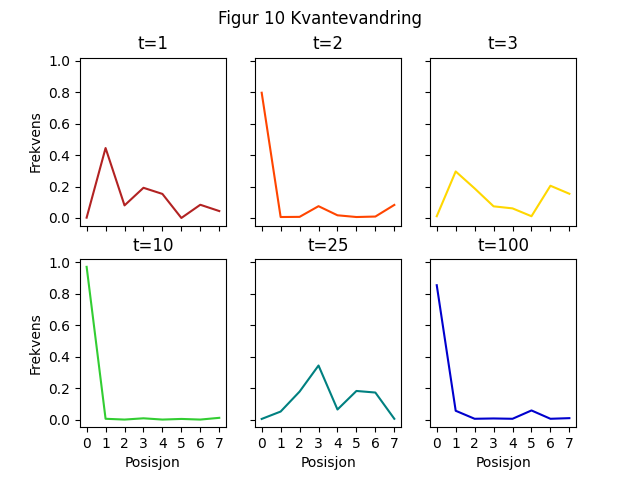
\includegraphics[scale=0.5]{Fig10Start0.png}
                        \end{center}
                    \end{subfigure} \\
                    \begin{subfigure}{0.6\textwidth}
                        \begin{center}
                            \caption{start uniformt}
                            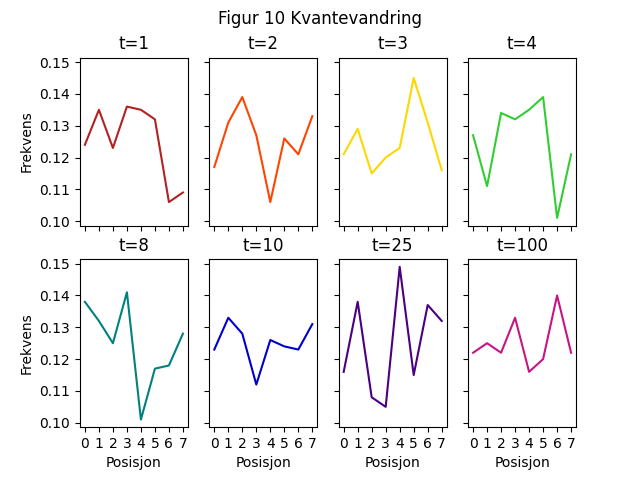
\includegraphics[scale=0.5]{Fig10Hadamard.png}
                        \end{center}
                    \end{subfigure}
                    \label{fig:shuriken vandring}
                \end{center}
            \end{figure}
       
        \subsubsection{Staggered model}

            For kvantevandringen vi utfører på denne modellen har jeg ikke klart å lage en implementasjon som gir meg ønsket kvantevandring. Den implementasjonen som man kan finne på repoet, gir desverre en annen kvantevandring, enn den som er spesifisert tidligere i rapporten. Dette eksempelet er derimot beholdt, ettersom vi bruker denne vandringen for å illustrere QSS. Den abstrakte implementasjonen ligger fremdeles under, og her foregår kvantevandringen over Hilbertrommet $\mathcal{H}_V$, representert som \emph{position}.
                
            \begin{Verbatim}[gobble=2, numbers=left, frame=lines,
                framesep=3mm,
                label={[Beginning of code]End of code}]
                // The staggering is determined by the chosen graph tessellation cover
                operation StaggeredWalk(position : Qubit[], 
                                        Staggering : (Qubit[] => Unit is Adj), 
                                        steps : Int) 
                                        : Unit is Adj {
                    for i in 1..steps {
                        Staggering(position);
                    }
                }
            \end{Verbatim}

            Denne vandringen er definert unikt utifra graftesselleringsdekket som er valgt. Det er operatoren Staggering som skal være den unitære vandringsoperatoren som er definert slik. Vi kan se på kvantevandringen som er implementert. Vi ser i dataen for den i figur \ref{fig:shuriken vandring} at vi har de samme tilfeldige mønstrene. I (a) hinter det sterkt til at vi har en quasi-periodisitet på $2$, ettersom den samler seg tilbake i node 0 for hvert partall.

            I (b) av figur \ref{fig:shuriken vandring} blir det åpenbart at kvantevandring som er implementert ikke stemmer overens med den som er spesifisert. Hvis vi husker operatoren $U$ som er komposisjonen av de tre hermitiske operatorene, så er det denne operatoren som skal implementeres. For å implementere $U$ trenger vi å beskrive $U$ som en komposisjon av de universelle unitære operatorene. Dette problemet kalles for unitær dekomponering. På denne fronten er det funnet mange resultater, blant annet at en generell dekomponeringsalgoritme kan ikke være bedre enn $\mathcal{O}(4^n)$ porter, hvor $n$ er antallet qubits. $ZYZ$-dekomponering er en simpel algoritme, men har ikke så god ytelse i forhold til denne nedre begrensingen. Optimalisert Shannon dekomponering ligger derimot på den teoretiske nedre begrensingen for små qubits \cite{krol2021efficient}. For denne implementeringen bruker vi Python pakken utviklet av Dmytro \cite{article}. Denne pakken har som hovedfunksjonalitet ved å generere Q\# kode gitt en unitær matrise.

            Måten vi ser at denne kvantevandringen ikke følger spesifikasjonene sine gjør vi ved å finne fikspunkter til operatoren $U$. En av disse fikspunktene er vektoren $H^{\otimes 3}|0\rangle$, altså at $U\circ H^{\otimes 3}(|0\rangle)=H^{\otimes 3}|0\rangle$. Vi kan enkelt observere at i figur \ref{fig:shuriken vandring} (b) at $t=1$ og $t=2$ ikke er det samme plottet, og dette bryter med observasjonen av fikspunktet. Tulsi sin beskrivelse av kvantesøk \cite{PhysRevA.86.042331} sier at vi fremdeles kan bruke denne operatoren som en kvantevandrings operator, og dette er grunnen for at vi overseer denne feilen.



            \begin{figure}
                \begin{center}
                    \caption{QSS søk over \ref{fig:shuriken}, med tidligere kvantevandring}
                    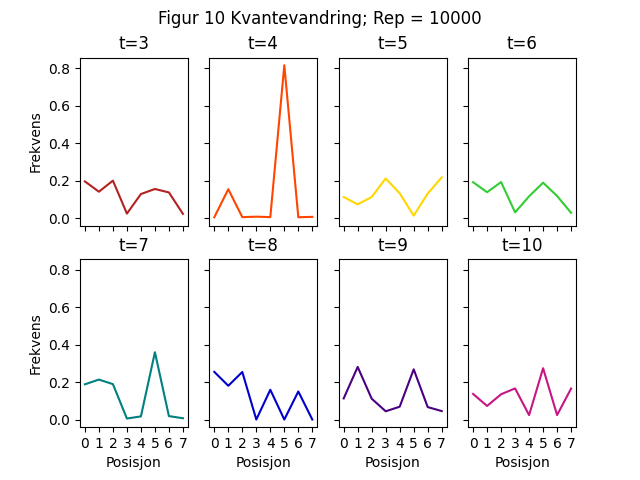
\includegraphics[scale=0.5]{Fig10QSSAmp.png}
                    \label{fig:QSS}
                \end{center}
            \end{figure}
        
    \subsection{Kvantesøk}

        Vi illustrer et eksempel av QSS algoritmen. Denne delen har som formål med å illustrere hvordan man kan gjøre den nødvendige forhåndsanalysen, og vise en mulig implementasjon av en slik søke algoritme. Den abstrakte søke algoritmen er gitt under.

        \begin{Verbatim}[gobble=2, numbers=left, frame=lines,
            framesep=3mm,
            label={[Beginning of code]End of code}]
            // Quantum Search
            operation QuantumSpatialSearch(register : Qubit[],  
                                            quantumWalk : (Qubit[], Int) => Unit is Adj, 
                                            phaseOracle : Qubit[] => Unit is Adj, 
                                            steps : Int, 
                                            weight : Int) 
                                            : Unit is Adj {
                // Spatial Search
                for i in 1..steps {
                    phaseOracle(register);
                    quantumWalk(register, weight);
                }
            }
        \end{Verbatim}

        Vi skal illustrere QSS algoritmen på figur \ref{fig:shuriken}, med graftesselleringsdekket som er gitt. For dette QSS eksperimentet skal vi anta at den 5 noden er merket, det vil si at det er den noden som vi skal nå fram til. La $\psi(t) = U^t(\psi(0)) = U^t(H^{\otimes 3}|0\rangle)$ være tilstanden til systemet ved tid $t$. Sjansen for å måle node 5 er dermed $p(t) = |\langle 5|\psi(t)\rangle = \langle 5|U^t(\psi(0))\rangle$. Om vi finner den $t$-en som maksimerer denne funksjonen, så finner vi hvor lenge vi skal kjøre algoritmen. Her er det mange metoder man kan bruke, men det anbefales å numerisk tilnærme seg maksima. Vi går videre ved å bruke simplexalgoritmen, dette avslører at $t=5$ gir tilnærmet maksima, med $p(t) \approx 0,27$. For å forbedre denne sannsynligheten opp til $0,81$ kan vi bruke amplitudeforsterkningsteknikken. Ved å anta at $p(t) \approx 0,25$, får vi at $k = \lfloor \sfrac{\pi}{4\sqrt{p}}\rfloor \approx \lfloor\sfrac{2\pi}{4}\rfloor = 1$.

        I figur \ref{fig:QSS} illustrerer vi dette med kvantevandringen fra figur \ref{fig:shuriken vandring}. Siden denne operatoren er litt annerledes enn den som vi har spesifisert ender vi opp med maksimum på $t=4$. Ved å amplifisiere amplituden klarer vi øke den til $\approx 0.8$. Merk at på $t=7$ har vi enda en lokal maksima, og her kan man også bruke amplitudeforsterkningsteknikken for å gjøre det veldig sannsynlig å treffe node 5 etter måling.